\documentclass[12pt]{report}

\usepackage[utf8]{inputenc}
\usepackage[T1]{fontenc}
\usepackage[romanian,english]{babel}
\usepackage{geometry}
\usepackage{setspace}
\usepackage{amsmath}
\usepackage{graphicx}
\usepackage{pgfplots}
\usetikzlibrary{shapes.geometric, positioning, arrows.meta}
\usepackage{cite}
\usepackage[hidelinks]{hyperref}

\geometry{a4paper, margin=1in}
\pgfplotsset{compat=1.18}
\graphicspath{{images/}}
\onehalfspacing
\setlength{\parindent}{0pt}
\setlength{\parskip}{0.8em}
\begin{document}

\begin{titlepage}
    \centering

    {\large \textbf{UNIVERSITATEA BABEȘ-BOLYAI CLUJ-NAPOCA}\par}
    {\large \textbf{FACULTATEA DE MATEMATICĂ ȘI INFORMATICĂ}\par}
    {\large \textbf{SPECIALIZAREA INFORMATICĂ ENGLEZĂ}\par}

    \vspace{4cm}

    {\Huge \textbf{LUCRARE DE LICENȚĂ}\par}

    \vspace{2cm}

    {\LARGE \textbf{Moons \& Stars: A Game with Procedurally Generated Planets}\par}

    \vfill

    \begin{flushleft}
        \large \textbf{Conducător științific}\\
        Lect. Dr. Mircea Ioan Gabriel
    \end{flushleft}

    \vspace{1cm}

    \begin{flushright}
        \large \textit{Absolvent}\\
        Ábel Ujfalusi
    \end{flushright}

\end{titlepage}
\newpage
\thispagestyle{empty}
\mbox{}
\newpage

\chapter*{Abstract}

This thesis describes the creation of the video game Moons\&Stars, a space exploration and shooter game that features procedurally generated planet, giving it a unique game world. The players can interact within a completely procedurally generated universe, that will give the game an infinite number of possible worlds to play in, while also eliminating the need for manual content creation.

There were many challenges that had to be tackled during the creation of the game. This paper goes through the solutions given to these challenges and also discusses why each of them was chosen in order to tackle that given problem instead of other alternatives. It will discuss topics related to procedural generation, sphere creation, implementing a level of detail system, texture mapping and networking for multiplayer.

The main focus and biggest challenge of the work is the planet generation system. While exploring multiple options for the generation of spheres, the cube-sphere method is selected for its simplicity and for its ability to be easily subdivided or merged back for the application of level-of-detail techniques. The level of detail system makes use of quadtrees in order to efficiently facilitate the changes between resolutions in real time on the parts of the visible sphere being closest to the viewing camera. In order to form the simple spheres into unique and realistic looking planets with realistic looking terrain, Perlin-noise and other mathematical algorithms are applied over the spheres. Different simple mathematical functions are explored in order to create the shapes needed to form the terrain from the spheres.

\newpage
\tableofcontents
\newpage

\chapter{Introduction}
\section{Problem statement}

Games have been using procedural content generation (procedural generation, PCG) in the past \cite{pcgsmith2012, smelik2014} in order to create vast randomized worlds that players can enjoy a long time, while also cutting down on modeling and texturing work \cite{hendrikx2013}. Games such as \textit{No Man's Sky} or \textit{Minecraft} and many others have demonstrated the successful use and viability of the technique already in commercial games. Procedural content generation is used also in many other ways to enhance gaming experience, such as creating unique narratives and stories, resource instantiation and in many other ways. Use of procedural generation became even more common the past years due to the ever growing demand of more content inside video games and the financial challenges of creating enough content for these games \cite{hendrikx2013, 1118424ar}. 

From this challenge of filling the need for ever more content that is also becoming more detailed new techniques to generate this content procedurally arose as well \cite{korn2017game}. In the last years modern game engines like Unreal Engine or Unity reduced the needed code and its complexity significantly. Data reflects a clear shift from the main constraint being cost of engineering to becoming cost of visuals and assets \cite{serpa2019towards, martins2026financial}. A recent industry breakdown based on data from popular games and industry leading studios can be viewed in  Figure~\ref{fig:budget_breakdown}

\begin{figure}[htbp]
\centering
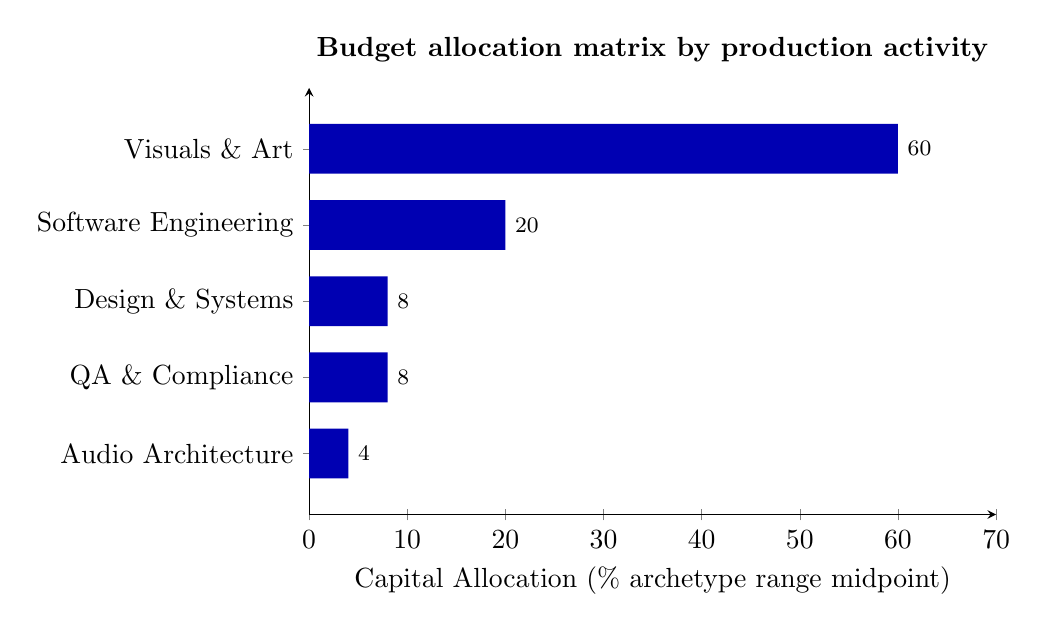
\begin{tikzpicture}
\begin{axis}[
    xbar,
    width=0.85\textwidth,
    height=7cm,
    xmin=0, xmax=70,
    xlabel={Capital Allocation (\% archetype range midpoint)},
    symbolic y coords={Audio Architecture, QA \& Compliance, Design \& Systems, Software Engineering, Visuals \& Art},
    ytick=data,
    nodes near coords,
    nodes near coords align={horizontal},
    every node near coord/.style={font=\footnotesize\bfseries, color=black},
    axis x line=bottom,
    axis y line=left,
    enlarge y limits=0.2,
    bar width=18pt,
    title={\textbf{Budget allocation matrix by production activity}}
]
\addplot[fill=blue!70!black, draw=none] coordinates {
    (60,Visuals \& Art)
    (20,Software Engineering)
    (8,Design \& Systems)
    (8,QA \& Compliance)
    (4,Audio Architecture)
};
\end{axis}
\end{tikzpicture}
\caption{Distribution of internal development capital within flagship video game production pipelines, showing the absolute majority commanded by high-fidelity asset creation workflows.}
\label{fig:budget_breakdown}
\begin{spacing}{0.8}
\vskip 2mm
\noindent\footnotesize{\textbf{Sources:} Computed by the author based on aggregated cost frameworks from the \textit{Competition and Markets Authority Final Report} (2023, Paragraphs 7.42--7.55) \cite{cma2023videogames} and empirical case studies unredacted in \textit{FTC v. Microsoft Corp.}, No. 3:23-cv-02880-JSC (N.D. Cal. 2023) \cite{ftcvmicrosoft2023} detailing baseline production thresholds for high-fidelity interactive software (e.g., \textit{The Last of Us Part II} at \$220M and \textit{Horizon Forbidden West} at \$212M).}
\end{spacing}
\end{figure}

\newpage

\section{Motivation}

This thesis is motivated to explore the foundations and use of such algorithms on spherical objects, with a very heavily varying level of detail, providing both an explorable universe of planets and playable individual worlds at the same time. It wants to find ways to generate assets and game worlds for use without costly manual modelling of 3D assets. The use of procedural generation in space games have been explored before but their use in multiplayer, small indie creations remains limited. 

This work implements procedural planet generation inside a small indie creation, inside a strictly multiplayer creation and to analyze the techniques viability in small scale multiplayer creations. The goal was developing an enjoyable multiplayer game with minimal texturing and modelling work done. This reduction in assets can make it possible for very small scale teams, or even single creators, possible to create commercial quaility games.

\section{Challenges}

The first challenge to be tackled in this work is the generation of a single sphere. Multiple sphere generation methods are explored, each with their drawbacks and advantages \cite{doliveira2018} . It takes careful consideration to choose from the plethora of ways a single sphere can be generated and will be very impactful down the line when it comes to the implementation of other systems, such as the level of detail or terrain generation.

The second problem is implementing a sufficiently fast and efficient level of detail system that can provide enough details close up for the planets to be actually playable, but will be able to successfully reduce resolution to a level where a far away overview from space will not be too much burden on regular hardware.

Then the most important part in order to obtain randomized planets with realistic looking geometry will be the application of Perlin-noise with various tweaks introduced. In order to generate the shape imitating real-world geologic features, we will combine Perlin-noise layers with other simple mathematical functions that will give more detail to it.

Finally, these procedurally generated planets will be placed into a complete game world, in a space shooter where players can play against each other.

\section{Previous work}

The application of procedural content generation within commercial game architectures has evolved from an early optimization strategy to a potential fundamental design paradigm. As outlined in the comprehensive survey made by Hendrikx et al. \cite{hendrikx2013}, PCG can be employed across multiple layers of virtual environments: ranging from low-level geometric data to high-level systemic mechanics. The primary driver for modern PCG integration is the mitigation of skyrocketing production costs associated with high-fidelity asset modeling \cite{smelik2014}. Traditional development structures increasingly struggle under the financial burden of manual asset creation, allowing algorithmic synthesis to bridge the resource gap for independent developers who require expansive virtual ecosystems \cite{short2017, korn2017game}. Early foundational mechanics demonstrated by Smith et al. \cite{pcgsmith2012} confirm that when PCG is integrated directly into the core gameplay loop, it can completely redefines spatial exploration and player strategy.

The core challenge of rendering large scale procedural words is the efficient management of compute and memory resources while also providing the player with pleasing visuals. This requires dynamic level of detail (LOD) systems. The conceptual foundation of hierarchies with multiple resolutions was introduced by Clark \cite{clark1976}, establishing that computation times should scale linearly with visible scene complexity rather than total world geometry. For heightfield rendering and expansive terrain structures, continuous LOD algorithms became standard, allowing seamless mesh transitions to prevent visual popping artifacts \cite{lindstrom1996}. Modern implementations have migrated these approaches onto modern hardware architectures, exploiting GPU-based continuous chunk allocations to optimize real time performance thresholds \cite{hugues2005, Wang2020LevelOD}. In contemporary engine pipelines, these systems rely heavily on quadtree data structures to dynamically subdivide terrain nodes based on their distance to the player camera \cite{wu2010, deaconu2021}.

Shifting to a sphere geometry from flat terrain often causes distortion if algorithms aren't carefully selected or adapted. Consequently, specific research has focused on alternative grid arrangements, such as the development of novel coordinate systems for constructing balanced spherical grid topologies \cite{lei2020}. To establish cohesive multi-resolution terrain directly on these spherical models, d'Oliveira and Apolinario Jr. \cite{doliveira2018} successfully adapted planetary-scale multi-resolution frameworks tailored for real-time video games. This structural combination allows developers to reconcile macroscopic celestial navigation with localized, high-fidelity ground interaction. A recent comparative analysis by Zechmann and Hlavacs \cite{zechmann2025} systematically evaluates modern procedural planet generators, highlighting the performance tradeoffs between memory overhead and real-time generation speeds across different client architectures.

To inject naturalistic complexity into these spherical meshes, stochastic noise algorithms are universally applied to simulate geological patterns. The historical baseline for this technique remains Perlin noise, introduced by Ken Perlin \cite{perlin1985} to synthesize pseudo-random textures through coherent gradients. This was later optimized into Simplex noise to correct second-order interpolation discontinuities and gradient distribution issues \cite{perlin2002}. Within contemporary terrain pipelines, these noise variants are layered fractally via octaves, altering the overall landscape roughness and lacunarity \cite{rose2016}. As documented in a recent literature review on the evolutionary trajectory of Perlin noise and its mathematical improvements \cite{wu2024}, modern pipelines routinely combine these gradient noise functions with secondary mathematical filters to accurately mimic authentic tectonic and erosive formations.

\newpage

\chapter{Theoretical foundations}

This chapter will present the theoretical concepts and foundations the work is built on and also existing research in the field. It covers procedural generation techniques, their possible applications, different ways of sphere generation and the mathematical principles behind Perlin noise, the main tool for generating randomized terrains. It also covers the quadtree data structure and level of detail algorithms that employ it. Finally, it takes a look at a simple way of providing texture for the created meshes. Understanding of these concepts is essential in order to make sense of the decisions made during the implementation of the works, discussed in the subsequent chapters.

\section{Procedural generation in games}

Procedural generation refers to any technique where creation of content happens through algorithms rather than manual work of humans \cite{short2017,rose2016,pcgsmith2012,hendrikx2013}. The technique is long used in video games and is also used in many of the most popular games of the market. It has many different uses that can enhance games in very different ways. It is also often used to provide infinite replayability in open ended games. 

\subsection{Types of procedural content}

Procedural content can be roughly categorized into several distinct type, each having a different purpose inside games \cite{pcgsmith2012, korn2017game}. First, most common use is the creation of game terrains, realistic or fantasy landscapes, any kind of playable world as place of player interactions. Use in level generation is also common, producing game levels, dungeons, or mission layouts, often filling them with procedurally generated loots and resources as well. Narrative generation is also often used for storytelling elements, giving uniqueness to the game's dialogues. Finally, texture and material generation is utilized in the production of terrain textures, surface details, unique and non-repeatable texturing of different objects.

This thesis focuses on terrain generation, more specifically terrain generation applied to spherical surfaces, and simple texture generation over those spherical words, inside a simple game world.

\subsection{Deterministic vs. stochastic generation}

A deterministic system is one where no randomness is involved in the development of future states of the system. In procedural content generation, this often refers to purely functional generation, for example the use of mathematical noise functions like Perlin where the output is a direct mapping of some input coordinate and/or seed value. Because the output is fixed for any given input, these systems are inherently reproducible, allowing for consistent world states given the same set of parameters, circumventing the need to save vast amounts of data about the generated world for reproducibility.

In contrast, stochastic generation introduces the element of chance and randomness. However, in computing today "randomness" refers to pseudo-random number generators in general. These generators while at first might look completely unpredictable still usually are made up of mathematical algorithms dependent on an initial seed value. Their output is governed by this initial seed value.

So in conclusion, most "random" game worlds are using the seeded-stochastic approach that appears endless, random looking content with the added benefit of easy reproducibility through a single seed value. The game presented in this work employs this method as well for the creation of its worlds.

\subsection{Level of detail systems}

The most critical challenge in rendering very large scale game environments is in the management of computing resources. Nearby objects need a high enough resolution to be detailed in a visually pleasing manner, but that is very computationally costly and also unnecessary for objects being far away from the viewpoint of the player's camera. Level of detail (LOD) systems have long been used \cite{clark1976} to address this by reducing the resolution of objects based on their distance from the camera \cite{wu2010,deaconu2021}.
For rendering worlds on a planetary scale an effective LOD system is essential, even more so to leverage the potential of infinite terrain generation possibilities given by procedural generation. There are many traditional ways to solve this problem of transitioning between different resolutions.

On of them is discrete LOD, where we use pre-defined models at varying complexity levels that swap based on distance. Can be very effective for static assets and computationally very lightweight but needs many models, generally all created by hand and is poorly suitable to be used alongside procedural generation;

A good alternative is a continuous LOD system, consisting of dynamic mesh simplification that adjusts the number of triangles inside a mesh in real-time \cite{lindstrom1996}. More complicated to implement and somewhat more resource-intensive but highly adjustable. It is also very suitable to be used alongside procedurally generated content;

A very interesting solution is geometry clipmaps, a technique for rendering large terrains using nested grids centered around the viewer \cite{hugues2005}. This technique, while very CPU-efficient because it treats terrain as a set of scrolling buffers, it can be memory-intensive as it maintains details in a fixed radius regardless of the camera's orientation. Furthermore, it is a technique designed to be used on flat planes, applying it to spheres will result in a serious amount of distortion at the poles.

These approaches are widely used in terrain rendering and have been adapted for planetary scale environments \cite{doliveira2018, korn2017game}.

For spherical geometry, these methods must be adapted to account for the closed surface topology, a challenge explored in detail in the following section \cite{zechmann2025}.

\section{Sphere mesh generation techniques}

Creating a sphere from triangles is a non-trivial problem in computer graphics. There are many different methods, each with very distinct advantages and trade-offs regarding the distribution of vertices, memory usage and suitability for subdivision-based LOD systems. The work reviews multiple options and also argues why the solution implemented in this work was chosen.

\subsection{UV sphere}

The UV sphere, also known as a latitude-longitude sphere, is constructed by arranging vertices in horizontal rings (latitudes) and vertical segments (longitudes). This method is conceptually simple and produces a regular grid-like structure governed by the following equation \ref{eq:uv_sphere_definition}:

\begin{equation}
\label{eq:uv_sphere_definition}
\begin{gathered}
    \mathbf{(x, y, z) = (r \sin \phi \cos \theta, \quad r \cos \phi, \quad r \sin \phi \sin \theta)} \\
    \text{where} \\
    \mathbf{\theta = u \cdot 2\pi} \quad \text{and} \quad \mathbf{\phi = v \cdot \pi}
\end{gathered}
\end{equation}

However, the UV sphere suffers from several significant drawbacks that heavily impacts its utility in procedural terrain generation. The first and biggest one is pole singularities: at the north and south poles, all meridians converge, creating triangles with increasingly poor aspect ratios \cite{lei2020}. This convergence leads to non-uniform vertex distribution: vertices are densely packed near the poles and sparsely distributed near the equator. This consequently also causes texture mapping distortion where the polar regions experience severe stretching when applying textures. These limitations make the UV spheres unsuitable for applications requiring uniform geometry, such as planetary terrain creation. 

\subsection{Icosahedral sphere}

The icosahedral sphere or icosphere, addresses the limitations of UV spheres by starting with a regular icosahedron - a polyhedron with 20 equilateral triangular faces — and than subdividing each triangle recursively. After the subdivisions, the vertices are normalized to lie on the unit sphere. This construction is governed by the recursive refinement and normalization process defined in Equation~\ref{eq:icosphere_definition}:

\begin{equation}
\label{eq:icosphere_definition}
\begin{gathered}
\mathbf{V_{new} = \text{normalize}\left(\frac{V_a + V_b}{2}\right)} \
\text{where} \
\mathbf{\text{normalize}(\mathbf{v}) = \frac{\mathbf{v}}{|\mathbf{v}|} \cdot r}
\end{gathered}
\end{equation}

In this context, $V_a$ and $V_b$ represent the vertices of an existing edge and $r$ denotes the desired radius of the sphere.

This approach offers several advantages compared to the more simple UV sphere \cite{doliveira2018,zechmann2025}. First it features a niform vertex distribution. All of the triangles remain roughly equal in size and shape across the entire sphere.
Second, it eliminates singularities, so unlike on the UV sphere, there are no poles or degenerate regions where vetices concentrate. It also offers good texture mapping properties. The uniform geometry minimizes distortion when applying surface details. While the icosphere is more suited for applications of procedural generation inside games, it still does suffer from a highly complex indexing and subdivision logic and is poorly suitable for a level of detail system.

\subsection{Cube sphere}

A cube sphere is generated by subdividing the faces of a cube and then projecting the vertices outward onto a sphere. This method produces a sphere with six distinct patches corresponding to the original cube faces. The initial cube structure used as the base geometry is illustrated in Figure~\ref{fig:cube_simple}. A simple sphere representation obtained from the cube is shown in Figure~\ref{fig:sphere_simple}.

\begin{figure}[h]
    \centering
    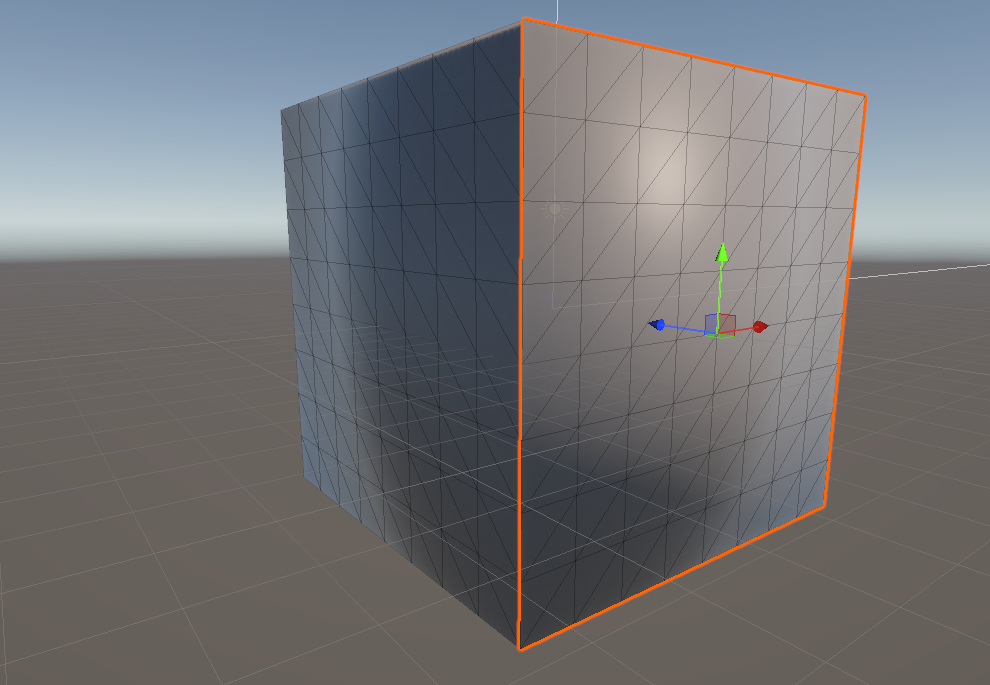
\includegraphics[width=0.5\textwidth]{cube_simple.png}
    \caption{Basic cube used as the starting point for cube-sphere generation}
    \label{fig:cube_simple}
\end{figure}

\newpage

\begin{figure}[h]
    \centering
    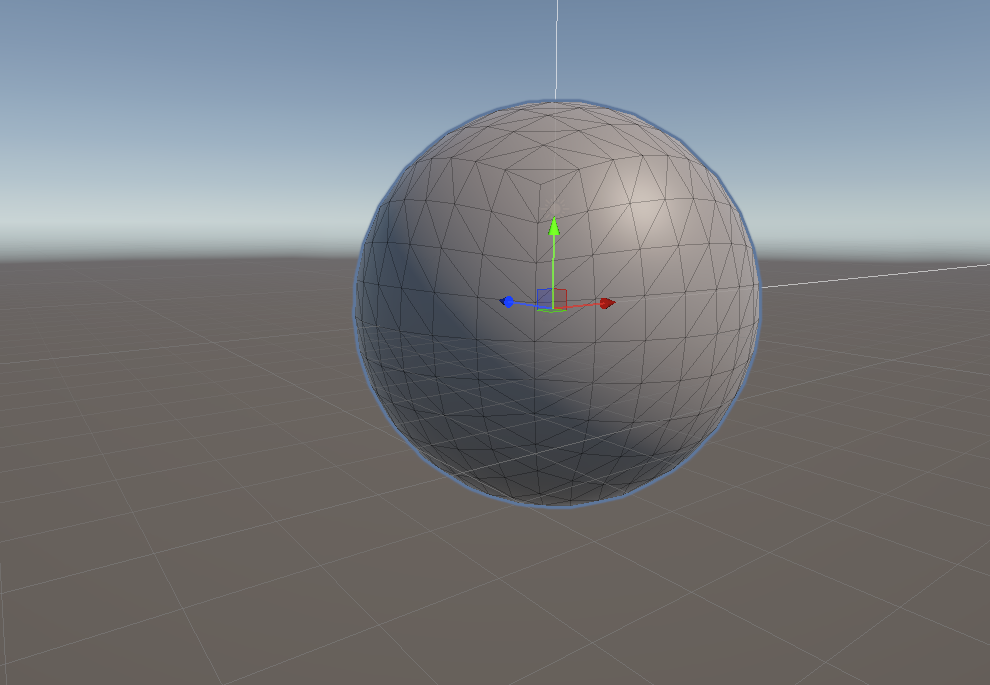
\includegraphics[width=0.5\textwidth]{sphere_simple.png}
    \caption{Simple sphere representation before applying terrain deformation}
    \label{fig:sphere_simple}
\end{figure}

The cube sphere offers a compromise between the UV and icosahedral approaches. By constructing the sphere from 6 faces, it avoids polar distortions entirely because each face retains a highly regular grid structure. Has no pole distortions, each face has a regular grid structure. More so, texture mapping is ver easy with this approach: each face can simply be treated as a 2D texture region. Furthermore, LOD implementation is a lot simpler due to this structure as well, quad-based subdivision can be applied uniformly across faces\cite{doliveira2018}. However, the cube sphere introduces visible seams along the edges of the six faces unless special care is taken to ensure smooth normals and consistent texture mapping at the boundaries.

For this thesis, the cubesphere approach was selected due to its uniform vertex distribution and natural compatibility with recursive subdivision for dynamic LOD systems.

\section{Perlin noise and procedural terrain}

To transform a mathematically perfect sphere into a realistic planet, elevation variations and surface details must be applied. Perlin noise, developed by Ken Perlin in 1983 for the film \textit{Tron}, provides the foundation for most procedural terrain generation systems \cite{wu2024}.

\subsection{Mathematical foundations}

Perlin noise is a gradient noise function that produces pseudo-random, coherent values over continuous space \cite{perlin1985}. Unlike pure random noise, Perlin noise exhibits smooth transitions between values, creating natural-looking patterns. The algorithm operates by firs defining a grid of integer lattice points with random gradient vectors. Than for any input point, identifies the surrounding lattice points, computes the dot product between each lattice point's gradient vector and the offset from that lattice point to the input point. Finally, it interpolates these values using a smoothsetp function to produce the final result. Figure~\ref{fig:perlin_noise} show image of Perlin noise output on grayscale.

Perlin's later work \cite{perlin2002} introduced \textit{Improved Perlin Noise}, which addressed artifacts in the original implementation by using a better interpolation function and a more robust gradient selection scheme.

\subsection{Octave summation}

Simple Perlin noise produces patterns at a single scale, which often appear too uniform. To create more natural, fractal-like terrain, multiple layers of noise, usally called octaves are summed together. Each successive octave has double the frequency and half the amplitude:

\[
f(\mathbf{p}) = \sum_{i=0}^{n-1} \frac{\text{noise}(2^i \mathbf{p})}{2^i}
\]

This summation, known as fractal Brownian motion (fBm), produces self-similar patterns at different scales, mimicking the multi-scale nature of real-world geologic features such as mountains, hills, and rocks.

\begin{figure}[h]
    \centering
    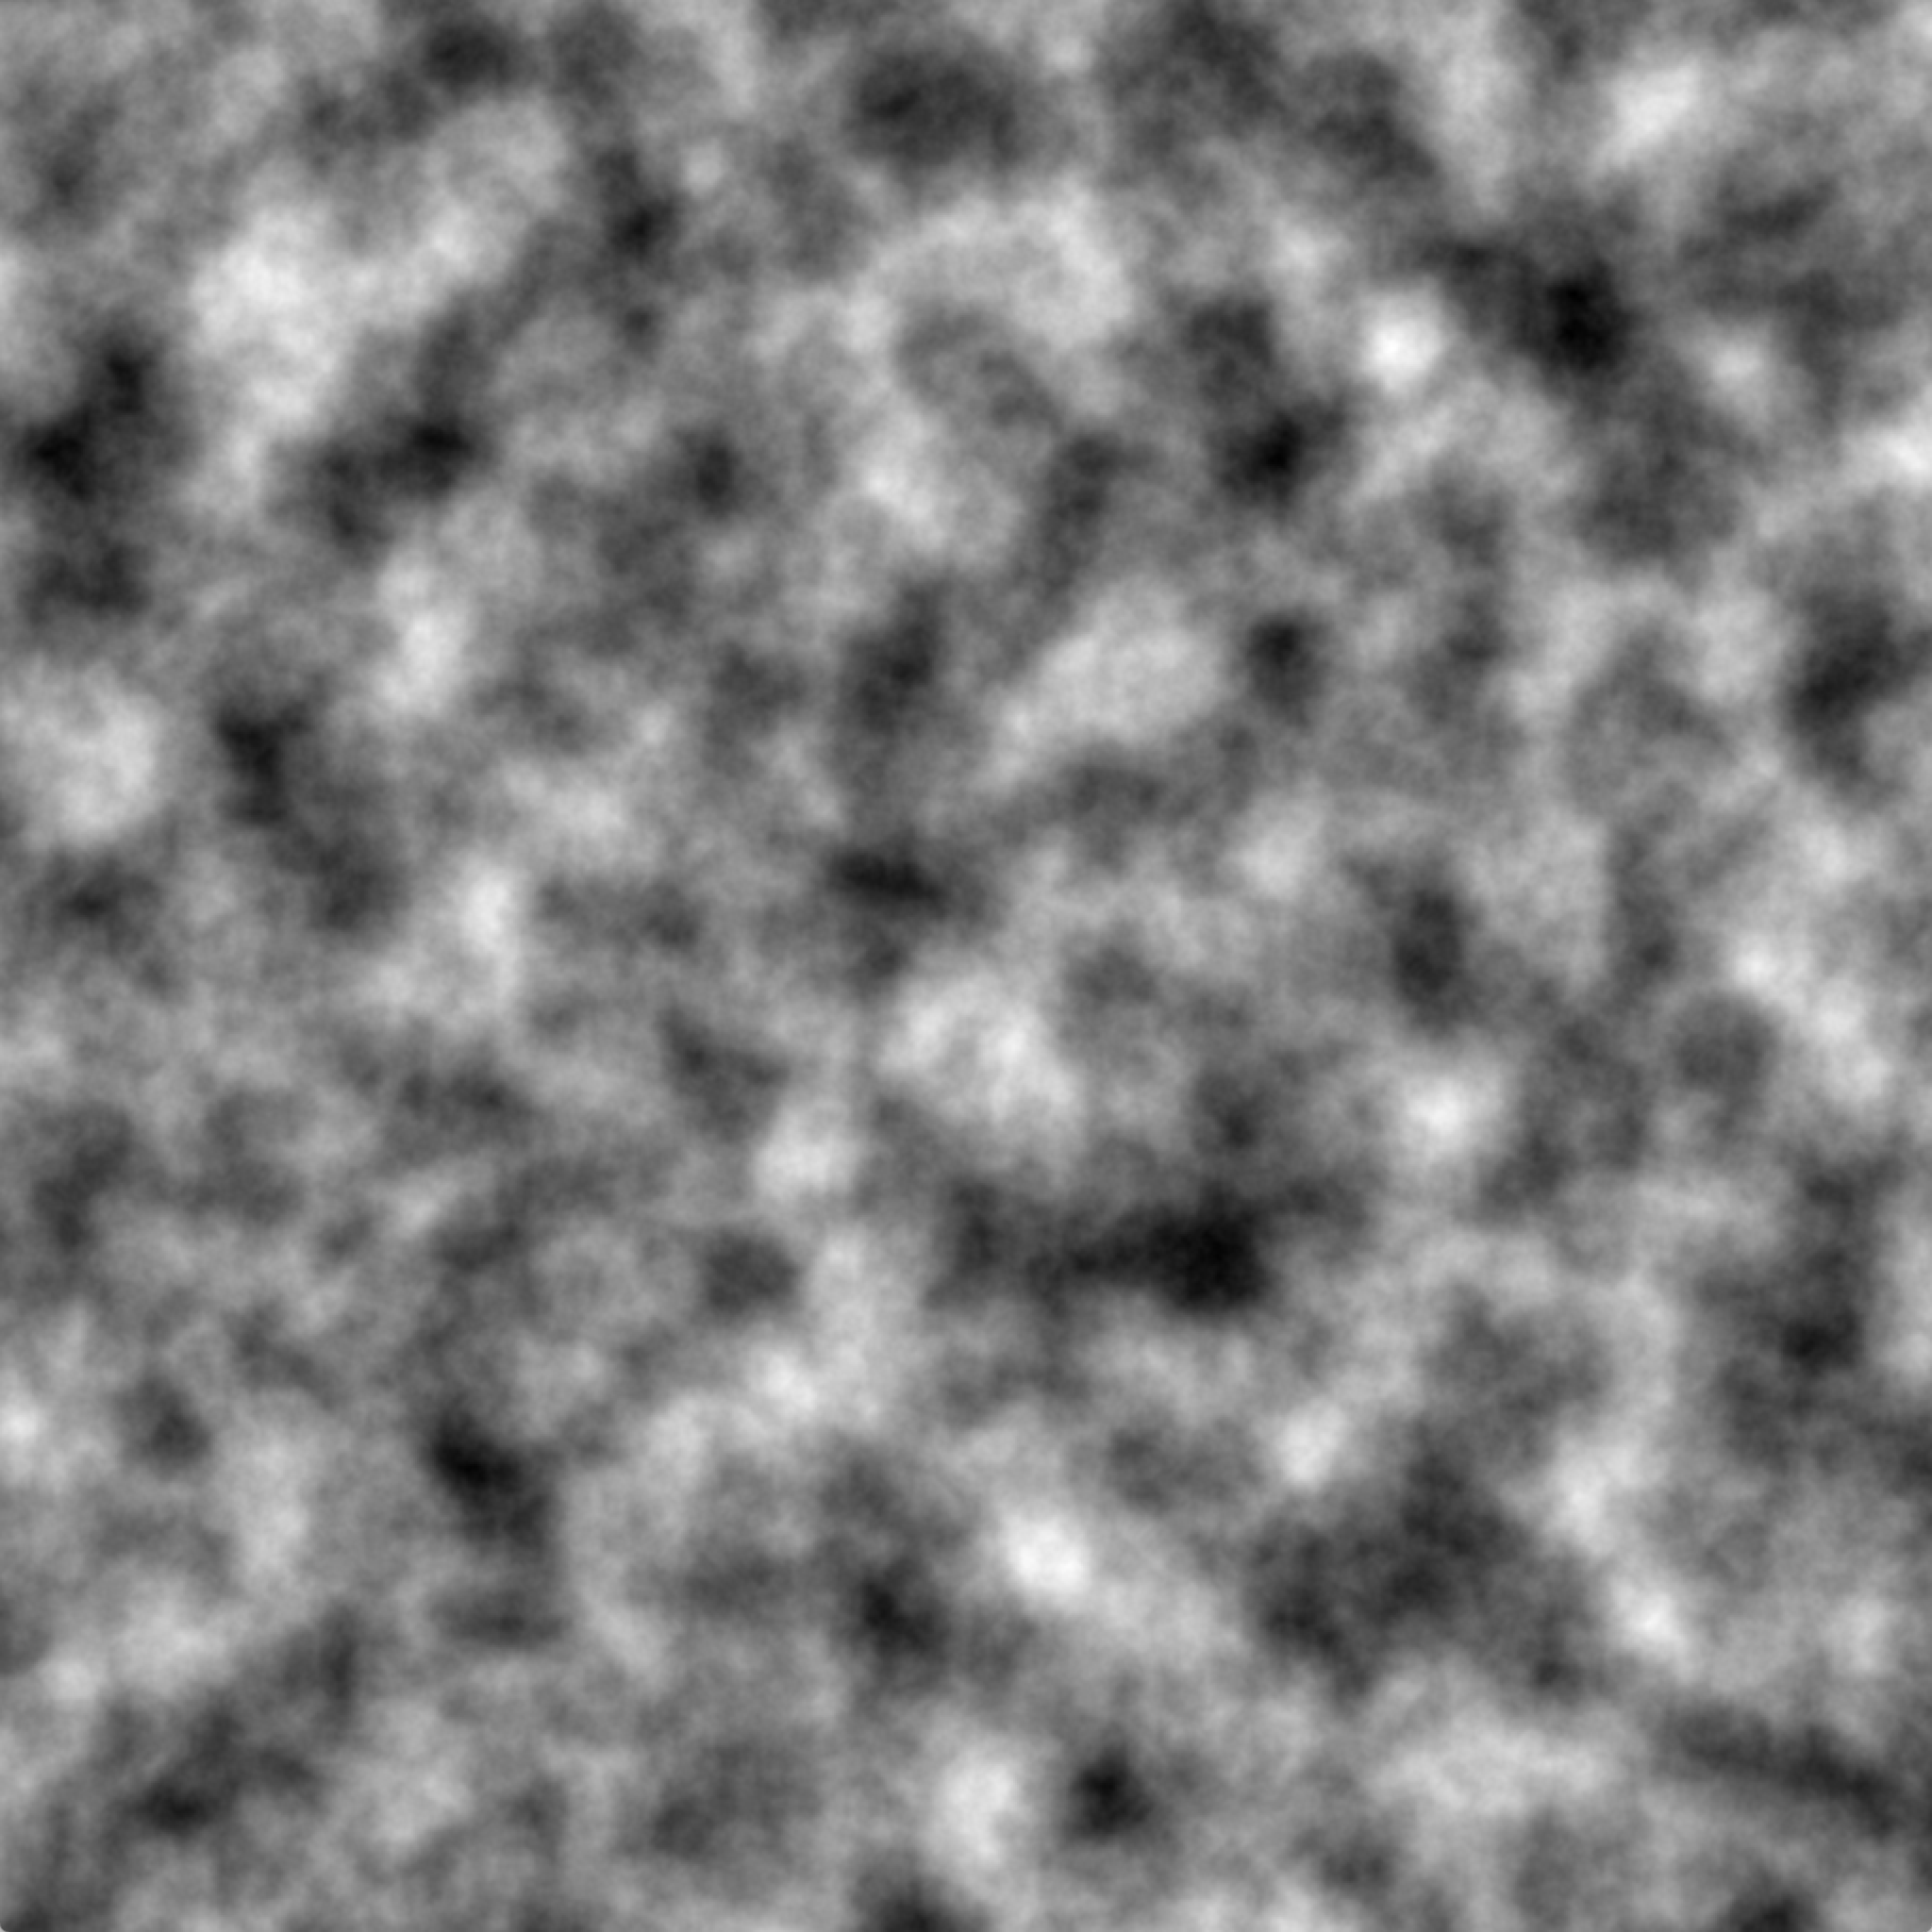
\includegraphics[width=0.6\textwidth]{perlin.png}
    \caption{Perlin noise as grayscale image}
    \label{fig:perlin_noise}
\end{figure}

\subsection{Applications to planetary generation}

For generating planets, Perlin noise can be applied for multiple parts to dynamically shape the entire world \cite{hendrikx2013, doliveira2018, zechmann2025, korn2017game}. First, using 3D noise for terain elevation. Three-dimensional noise functions on the sphere's surface coordinates the continuous terrain elevation data. Another great use is biome distribution, different noise functions can determine climate zones, moisture levels, and biome types accross the planet. Then elevation, slop and biome information already generated with the help of Perlin noise can be combined in order to assign surface colors to the planet. Lastly, noise functions can also help determine the placement of any other objects that give additional detail to the planet, like rocks, trees and other similar features. By combining multiple noise functions with different frequencies and amplitudes, a wide variety of planet types can be created from simple barren rock, to lush worlds with intricate biomes and vegetation.

\section{Quadtree data structure}

A quadtree is a hierarchical spatial data structure \cite{wu2010, zechmann2025} used to partition two dimensional space by recursively subdividing it into four equally sized regions. Each node in the tree represents a rectangular region defined by the coordinates of its 2 corners on a diagonal (called minimum and maximum coordinates). If higher detail is required in a region, the node is subdivided into four child nodes. Consequently, the 4 divided nodes can be merged back to 1 single node in a similar manner.

Quadtrees are particularly suitable for terrain rendering \cite{wu2010,deaconu2021, zechmann2025}, as they allow adaptive resolution depending on the viewer's position. Regions closer to the camera can be subdivided further, while distant regions remain at lower resolution.

In this work, quadtrees are applied to each face of the cube sphere representation. Each quadtree can have an associated mesh, making up a patch of the created planet. It will either contain a mesh patch or have 4 children. This enables efficient management of level of detail across the entire planetary surface. In addition, each quadnode can be independently hidden and not rendered easily with all its associated children in case it is invisible to the camera, saving further computing resources.

\section{Level of detail for planetary rendering}

Level of detail (LOD) techniques are essential when rendering planetary scale objects. A player may observe a planet from orbit or stand directly on its surface, requiring vastly different levels of geometric detail.

\subsection{Distance based LOD}

In this work, LOD is determined based on the distance between the camera and the surface patch. Each node computes the distance from the camera from its center. If camera distances shrinks, patches are subdivided after a given threshold and until a maximum given resolution. When the camera gets further, they are merged beack after leaving the resolution threshold. 

This approach ensures that nearby terrain is highly detailed while at the same time it simplifies distant objects and ensures that performance remains stable regardless of viewing scale.

\subsection{Subdivision and Merging}

The LOD system is defined by the basic operations of subdivision and merging. Each time a higher detail threshold is hit below the maximum resolution, subdivision happens and each node is divided into 4 child nodes. In the case of division the 4 child nodes are removed and replaced with a lower resolution parent mesh when detail is no longer needed. This dynamic process allows real time adaptation of terrain resolution as the player moves through the environment.

This hierarchical subdivision process applied on cube faces is illustrated in Figure~\ref{fig:cube_lod}, where different levels of detail are visible depending on the region. When level of detail is applied to spherical geometry, the resolution dynamically adapts depending on the camera distance, as illustrated in Figure~\ref{fig:sphere_lod}.

\begin{figure}[h]
    \centering
    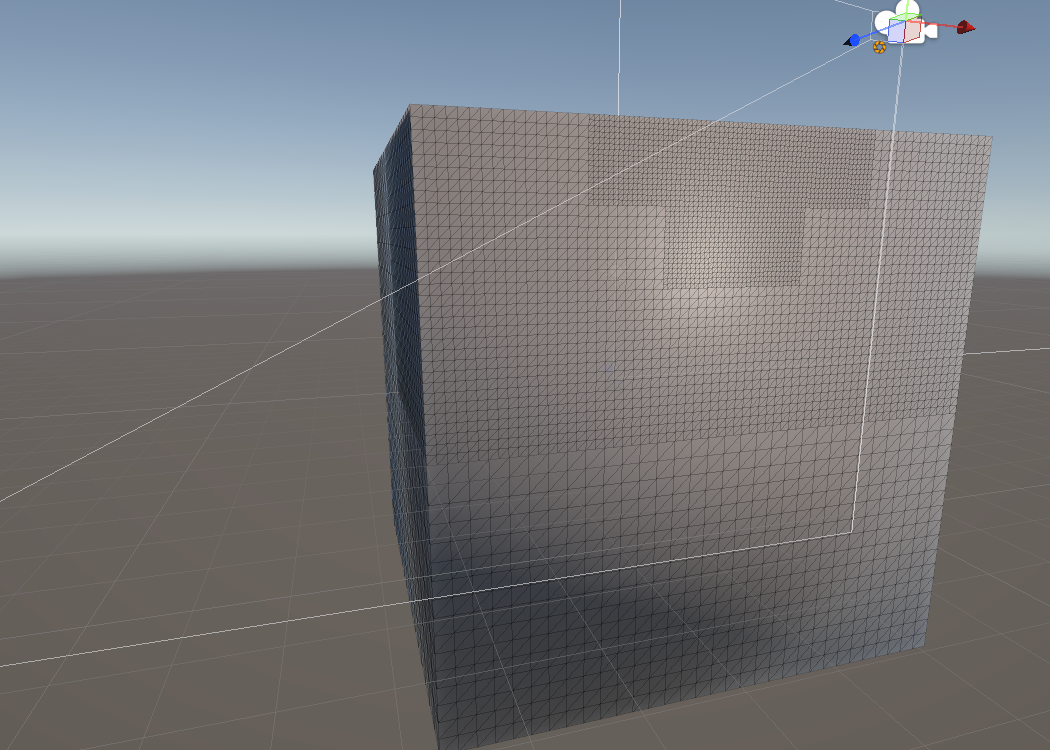
\includegraphics[width=0.6\textwidth]{cube_lod.png}
    \caption{Level of detail applied on cube faces using quadtree subdivision}
    \label{fig:cube_lod}
\end{figure}

\begin{figure}[h]
    \centering
    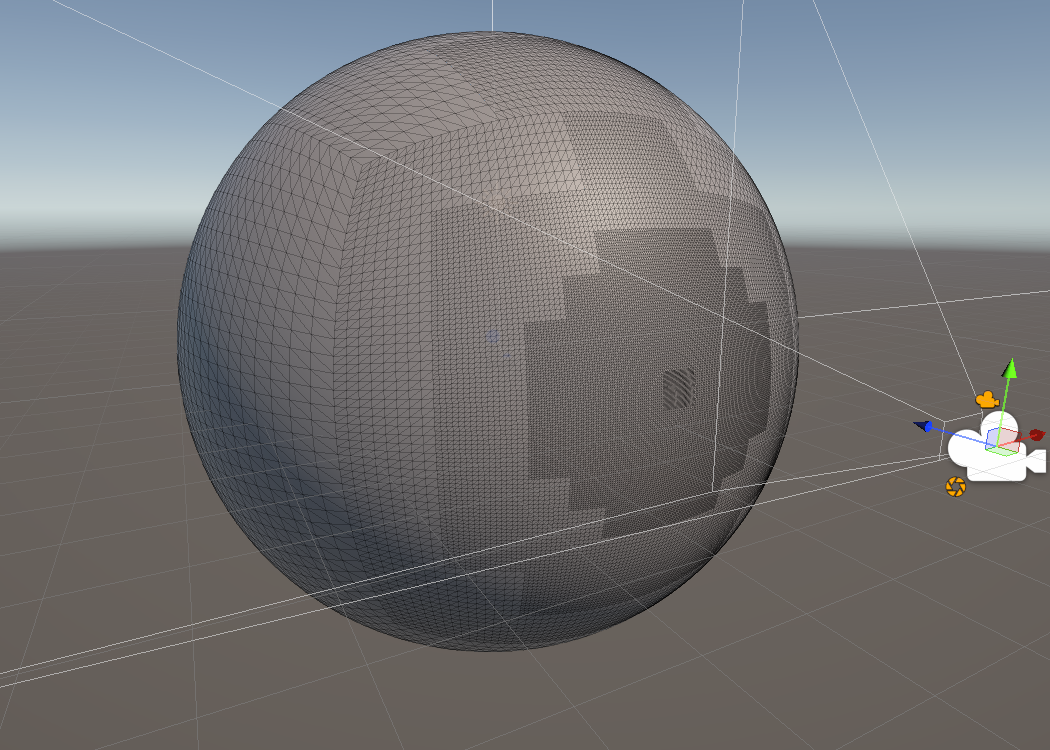
\includegraphics[width=0.6\textwidth]{sphere_lod.png}
    \caption{Level of detail applied on a sphere surface}
    \label{fig:sphere_lod}
\end{figure}

\section{Summary}

This chapter has examined the theoretical foundations necessary for implementing a procedurally generated planetary system. Procedural generation provides the framework for creating vast, deterministic and highly replayable virtual worlds, while sphere mesh generation techniques, more so in particular the cube sphere, offer the solid foundation for planet creation. Finally, Perlin noise and its fractal variants supply the mathematical tools for transforming simple spheres into realistic looking planets with surface details and textures.

\chapter{Planet generation system}

This chapter discusses in detail how one of the core features of the game, procedural planet generation will be implemented. Architectural decisions, reasoning behind them, sytem design and testing solutions for the planet generation are all discussed in this chapter, together with some possible performance improvements.

\section{Functional requirements}

The system must have provide 4 basic functionalities. Firstly, it must generate spherical objects at runtime. Secondly after that, these spherical objects must have dynamically adaptable resolution based on camera distance. Thirdly a terrain with variyng height levels should be applied over these spheres, generated with the help of Perlin noise. 
Forth and final requirement is that a texture scheme, with colors predefined by terrain height, must be applied over these planets for a visually striking appearance.

\section{System architecture}

The planet generation system can be subdivided into 2 big parts: first is mesh generation, while second is material and color generation. The 2 main subsystems interacting together will make up the planet generation.

\subsection{Mesh generation}

\bibliography{references}

\end{document}

